% Schematic representation of corona poling
% From NLO of organic molecules and polymers, Singh/Miyata.
% Author: Orlando Torres (2016)
\documentclass{standalone}
\usepackage{amsmath} % Required for \varPsi below
\usepackage{tikz,pgfplots}
\usetikzlibrary{calc}
\usetikzlibrary{patterns}
\tikzset{>=latex}
\begin{document}
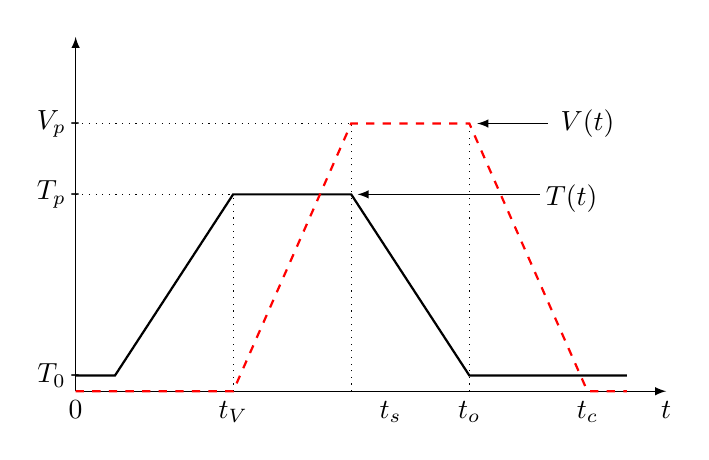
\begin{tikzpicture}

\coordinate (sg) at (5.9, 3);
\coordinate (sa) at (5.9, 3);

% horizontal axis
\draw[->] (0,0) -- (7.5,0) node[anchor=north] {$t$};
% labels
\draw	(0,0) node[anchor=north] {0}
		(2.0,0) node[anchor=north] {$t_V$}
		(4.0,0) node[anchor=north] {$t_{s}$}
		(5.0,0) node[anchor=north] {$t_o$}
		(6.5,0) node[anchor=north] {$t_c$};
% ranges


% vertical axis
\draw[->] (0,0) -- (0,4.5) node[anchor=east] {};
% labels
\draw	(0,0.2) node[anchor=east] {$T_0$}
		(0,0) node[anchor=south] {-}
		(0,2.5) node[anchor=east] {$T_p$}
		(0,2.3) node[anchor=south] {-}
		(0,3.4) node[anchor=east] {$V_p$}
		(0,3.2) node[anchor=south] {-}
		%(0,3.0) node[anchor=east] {$i_p$}
		%(0,2.8) node[anchor=south] {-}
		%(0,2.0) node[anchor=east] {$i_t$}
		%(0,1.8) node[anchor=south] {-}
		;

% graph edges
\draw[dotted] (2.0,0) -- (2.0,2.5);
\draw[dotted] (5.0,0) -- (5.0,3.4);
\draw[dotted] (0,2.5) -- (3.0,2.5);


%\draw[dotted] (6.5,0) -- (6.5,2.5);
%\draw[dotted] (2.5,2.5) -- (6.5,2.5);

%for voltage
\draw[dotted] (0,3.4) -- (3.5,3.4);
\draw[dotted] (3.5,0) -- (3.5,3.4);
%for current edges
%\draw[dotted] (0,3.0) -- (4,3.0);
%\draw[dotted] (0,2.0) -- (5,2.0);

% temperature
\draw[thick] (0,0.2) -- (0.5,0.2) -- (2.0,2.5) -- (3.5,2.5) -- (5.0,0.2) -- (7,0.2);
% voltage
%\draw[thick,dashed,color=red] (0.0,0.0) -- (2.0,0.0) .. controls (2.0,3.4) and (3.5,3.4) .. (4.0,3.4) -- (5,3.4) .. controls (5,0.2) and (6.5,0.0) .. (7.0,0.0);
\draw[thick,dashed,color=red] (0.0,0.0) -- (2.0,0.0) -- (3.5,3.4) -- (5,3.4) -- (6.5,0) -- (7.0,0.0);
% current
%\draw[thick,dashdotted,color=blue] (0.0,0.0) -- (2.0,0.0) .. controls (2.0,3.0) and (3.5,3.0) .. (4.0,3.0) -- (4.0,3.0) .. controls (4,2.7) and (4.5,1.9) .. (5.0,2.0) -- (5.0,2.0) .. controls (5.3,0.2) and (6.8,0.0) .. (7.0,0.0);

\draw [<-] ($(sg) - (0.8, -0.4)$) -- ($(sg) + (0.1, 0.4)$);
\draw (sg) node (sg) at +(0.6, 0.4) {$V(t)$};

%\draw [<-] ($(sg) - (2.2, 0.4)$) -- ($(sg) - (0.25, 0.4)$);
%\draw (sg) node (sg) at +(0.1, -0.4) {$i(t)$};

\draw [<-] ($(sa) - (2.32, 0.5)$) -- ($(sa) - (0, 0.5)$);
\draw (sa) node (sa) at +(0.4, -0.55) {$T(t)$};

%\draw (1,1.5) node {$U_s$}; %label
%Y tick marks
%\foreach \x in {0,...,6}
%     		\draw (\x,1pt) -- (\x,-3pt)
%			node[anchor=north] {\x};
%    	\foreach \y in {0,...,4}
%     		\draw (1pt,\y) -- (-3pt,\y) 
%     			node[anchor=east] {\y}; 
% Psis
%\draw[thick,dashed] (0,3) -- (2,3) parabola[bend at end] (6,1);
%\draw (2.5,3) node {$\varPsi_s$}; %label

\end{tikzpicture}

\end{document}